\chapter{Results}

\begin{comment}

Experiments:
- Explore the impact of capturing
    - Capturing NeRFs in different ways
        - Walking, standing still, sparsely, densely, linearly, around an object
    - Capturing video, images, polycam
        - Better/worse quality with polycam or COLMAP
    - Capturing different kind of scenes
        - Bounded/Unbounded 
    - Capturing in different conditions
    - Capturing 
    
- Explore the impact of dataset size
    - Extract different amounts of images from the video ✅
        - Simulate driving by walking up and back a street multiple times ✅
    - How much data is required until COLMAP becomes a bottleneck

- Explore the impact of area-size
    - Remember to point out that area is poorly defined since scale is perspective relative, depending on the level of detail you want. ✅
    - Area must be defined for a certain scene type. E.g. street view, aerial view, unbounded in multiple directions, bounded in all directions

- Explore the impact of different methods
    - instant-npg, nerfacto, NeRF

Metrics
- Quantitative
    - PSNR, LPIPS, SSIM
- Qualitative
    - Compare images side-by-side



Research questions:
- To what extent does a good capture impact the result of a NeRF
- How much data is required until COLMAP becomes a bottleneck?
- What is the capacity of a NeRF when optimizing a street view scene?

SCENES:
- Bounded scene
- Unbounded scene
- Walking
- Standing still
- Street-view
\end{comment}



\section{Dataset}
\begin{figure}[!h]
    \centering
    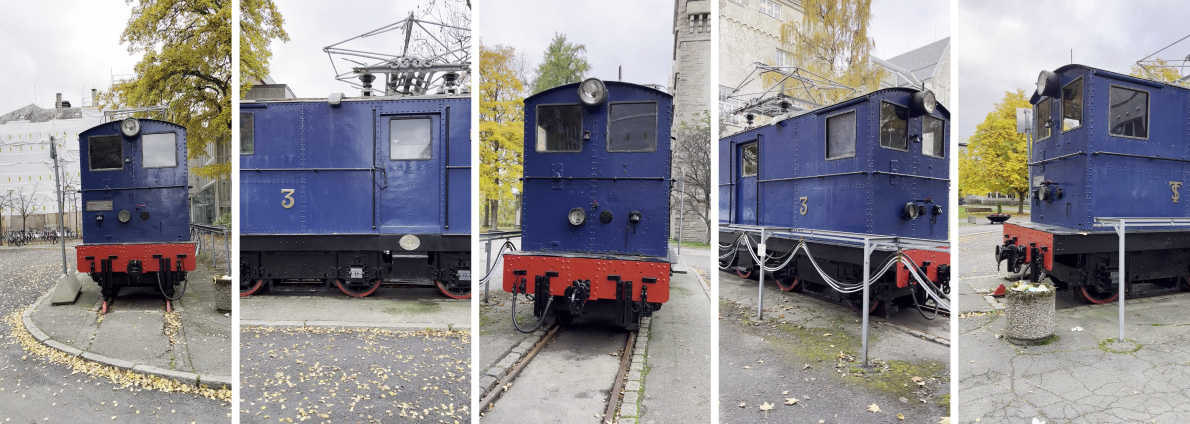
\includegraphics[width=1.0\textwidth]{figures/ohma_electra.png}
    \caption{Unbounded scene: The dataset of Ohma Electra is ~47 seconds long, captured at 30 FPS. The dataset contains 1416 images.}
    \label{fig:ohma-electra}
\end{figure}
\begin{figure}[!h]
    \centering
    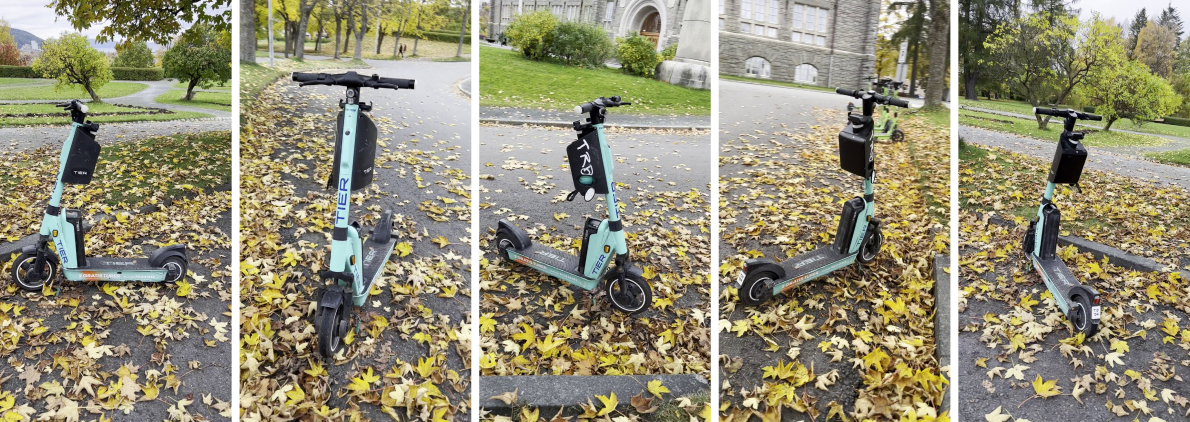
\includegraphics[width=1.0\textwidth]{figures/tier.png}
    \caption{Unbounded scene: The dataset of an electric scooter is ~15 seconds long, captured at 30 FPS. The dataset contains 446 images}
    \label{fig:tier}
\end{figure}

\begin{figure}[!ht]
    \centering
    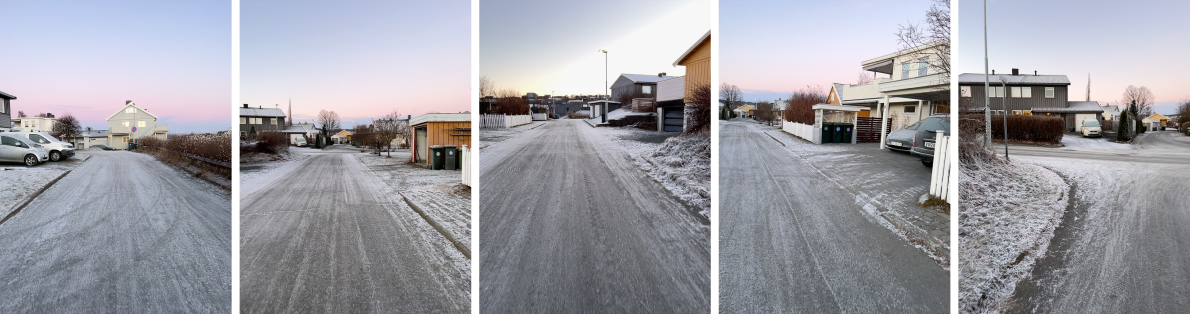
\includegraphics[width=1.0\textwidth]{figures/streetview-dataset.png}
    \caption{Large outdoor, unbounded scene: The dataset of a street in Trondheim is originally caught with the Polycam app. The dataset contains 600 images.}
    \label{fig:streetview-dataset}
\end{figure}
\begin{figure}[h]
    \centering
    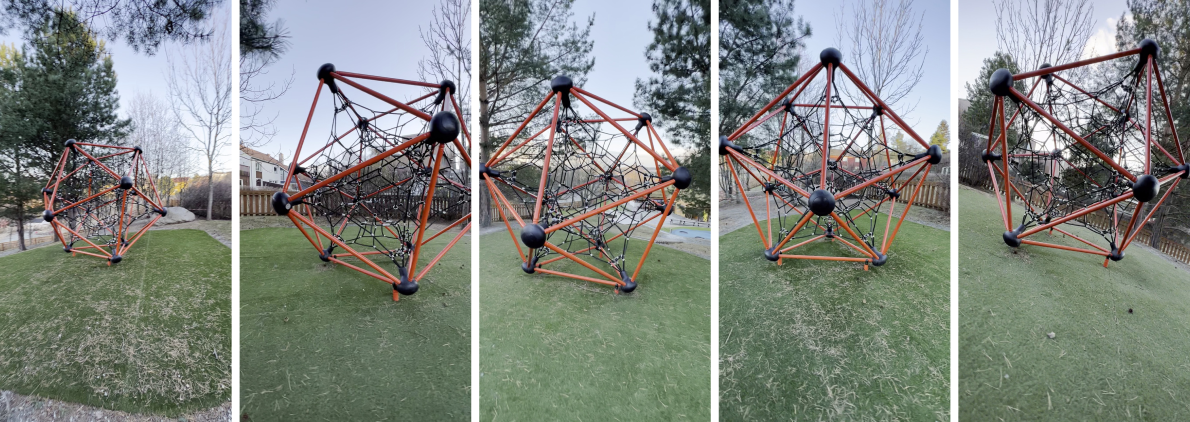
\includegraphics[width=1.0\textwidth]{figures/octahedron-dataset.png}
    \caption{Octahedron dataset. Caught with an iPhone at 0.5x zoom.}
    \label{fig:octahedron-dataset}
\end{figure}

\section{Dataset size}
We explore the impact of sampling different number of images from a video. The input video of Ohma Electra \cite{data:object-unbounded-ohma} is 47 seconds long, captured at 30 FPS resulting in 1410 total frames. Leveraging FFMPEG we sample frames at 4 increasingly dense levels.

\begin{comment}
\begin{table}[h]
\centering
\begin{tabular}{ccccccc}
\hline
\# Samples & PSNR $\uparrow$ & SSIM $\uparrow$ & LPIPS $\downarrow$ & Process Time & Training Time & Evaluate Time \\ \hline
5\%                       & 17.955    & 0.458     & 0.338    & 02:37    & 29:03    & 00:19    \\
10\%                      & 19.422    & 0.505     & 0.280    & 06:10    & 28:31    & 00:24    \\
15\%                      & 19.841    & 0.537     & 0.268    & 12:50    & 28:39    & 00:32    \\
20\%                      & 20.341    & 0.555     & 0.269    & 18:17    & 28:24    & 00:35    \\
25\%                      & 20.118    & 0.548     & 0.263    & 30:05    & 49:08    & 01:15    \\
40\%                      & 22.371    & 0.649     & 0.258    & 58:01    & 28:50    & 01:13    \\
50\%                      & 21.738    & 0.623     & 0.263    & -    & -    & -    \\
75\%                      & -    & -     & -    & -    & -    & -    \\
\multicolumn{1}{l}{100\%} & -    & -     & -    & -    & -    & -    \\ \hline
\end{tabular}
\caption{An overview of how dataset size impacts render-quality and process-, training- and evaluation-time. Trained on \autoref{fig:ohma-electra} with a vanilla Nerfacto pipeline}
\label{tab:colmap-dataset-size}
\end{table}
\end{comment}

\begin{table}[h]
\centering
\begin{tabular}{|l|llllll|}
\hline
\multicolumn{7}{|c|}{\textbf{Ohma Electra scene, \autoref{fig:ohma-electra}}} \\
\hline
\% Frames & PSNR $\uparrow$ & SSIM $\uparrow$ & LPIPS $\downarrow$ & Process & Training & Evaluate \\ \hline
20\%        & 19.692    & 0.523     & 0.272    & 00:36:55    & 20:40    & 00:44    \\
25\%        & 20.043    & 0.544     & 0.269    & 00:57:09    & 19:06    & 00:50    \\
33\%        & 20.135    & 0.547     & 0.273    & 01:22:08    & 20:15    & 01:05    \\
50\%        & 21.103    & 0.590     & 0.273    & 02:47:07    & 20:56    & 01:30    \\
100\%       & -    & -     & -    & -    & -    & -    \\
\hline
\end{tabular}
\caption{An overview of how dataset size impacts render-quality and process-, training- and evaluation-time. Trained on the ohma-electra dataset, as shown in \autoref{fig:ohma-electra}, with a default Nerfacto pipeline}
\label{tab:colmap-dataset-size}
\end{table}

Increasing the dataset size increases the amount of time required to retrieve the camera poses, given they're not known a priori. As discussed in \autoref{sec:colmap}, COLMAP has several different feature matching algorithms, e.g. exhaustive, sequential, and vocabulary tree matching. The choice of a matching algorithm should depend on the type of capture, e.g. if the source of the sampled images is a video it entails that subsequent frames have a certain overlap and makes sequential matching a sensible choice. The time complexity of COLMAP and its matching algorithms is important as the dataset size increases, as it might consume a lot of the time in the overall process-train-render pipeline. An overview of the selected matching algorithms' complexities can be seen in \autoref{tab:colmap-feature-complexity}.

\section{Area size}
We explore the impact of area size. Area in itself is poorly defined in the context of NeRF, since scale is perspective relative, depending on the level of detail you want. A single NeRF can efficiently represent a 3D model of the entire world, but the level of detail won't be satisfactory as you try to render detailed images. In this experiment we'll use a self-captured scene as the benchmark for area-related experiments. The scene \cite{data:streetview} is captured on a relatively straight street, bounded by houses on each side. 

\begin{table}[h] 
\centering
\begin{tabular}{ccccc}
\hline
Metric & 50m & 100m & 200m & 400m \\ \hline
PSNR   & -   & -    & -    & -    \\
LPIPS  & -   & -    & -    & -    \\
SSIM   & -   & -    & -    & -    \\ \hline
\end{tabular}
\label{tab:area-size}
\end{table}

\section{Different methods}
There are multiple different methods proposed for reconstructing 3D scenes and rendering novel views.

\begin{table}[h]
\centering
\begin{tabular}{|lcccc|}
\hline
\multicolumn{5}{|c|}{\textbf{Fox scene, \autoref{fig:fox-dataset}}} \\ 
\hline
Method  & PSNR $\uparrow$ & SSIM $\uparrow$ & LPIPS $\downarrow$& Time  \\ 
\hline
NeRF        & -    & -     & -    & -    \\
mip-NeRF    & -    & -     & -    & -    \\
instant-ngp & 26.370    & 0.863     & 0.214    & 47:45    \\
Nerfacto    & 27.698    & 0.859     & 0.190    & 31:28    \\
\hline

\hline
\multicolumn{5}{|c|}{\textbf{Ohma Electra scene, \autoref{fig:ohma-electra}}} \\ 
\hline
Method  & PSNR $\uparrow$ & SSIM $\uparrow$ & LPIPS $\downarrow$& Time  \\ 
\hline
NeRF        & -    & -     & -    & -    \\
mip-NeRF    & -    & -     & -    & -    \\
instant-ngp & -    & -     & -    & -    \\
Nerfacto    & 20.135    & 0.547     & 0.273    & 20:15    \\ 
\hline

\hline
\multicolumn{5}{|c|}{\textbf{Lego scene, \autoref{fig:ohma-electra}}} \\ 
\hline
Method  & PSNR $\uparrow$ & SSIM $\uparrow$ & LPIPS $\downarrow$& Time  \\ 
\hline
NeRF        & -    & -     & -    & -    \\
mip-NeRF    & -    & -     & -    & -    \\
instant-ngp (Default)     & -    & -     & -    & -    \\
instant-ngp (Adjusted)     & 33.854    & 0.969     & 0.0128    & 21:56    \\
Nerfacto (Default)    & 8.922    & 0.576     & 0.586    & 28:39    \\ 
Nerfacto (Adjusted)    & 19.544    & 0.759     & 0.113    & 28:05    \\ 
\hline
\end{tabular}
\caption{Same scene pre-processed in the same way with the default amount of frames and trained for equal amounts of epochs.}
\label{tab:method-comparison}
\end{table}




\section{Capturing}
\subsection{Polycam vs. COLMAP}
%- Run COLMAP on the images captured from Polycam. Compare the results.

\begin{table}[h]
\centering
\begin{tabular}{lcccc}
\hline
Method  & PSNR $\uparrow$ & SSIM $\uparrow$ & LPIPS $\downarrow$& Time  \\ \hline
%COLMAP - Sequential         & -    & -     & -    & -     \\
%COLMAP - Vocabulary tree    & -    & -     & -    & -     \\
COLMAP - Exhaustive         & 20.408    & 0.520    &  0.431     & 154:33     \\
Polycam                     & 21.488    & 0.544    & 0.413      & 00:11 \\
\hline
\end{tabular}
\caption{Using the corrected camera poses from Polycam renders better results on all metrics, and is significantly faster than calculating the camera poses with COLMAP after the capture.}
\label{tab:colmap-polycam-comparison}
\end{table}



% From Discord thread
\begin{comment} 
\textbf{Wavy artifacts in Nerfacto:}
AFAIK those wavy artifacts are from how the nerfacto model does ray sampling. Sometimes for very thin objects, none of the samples across a ray will land on it, causing it not to be visible in the rendering 

\textbf{Better results with another model?}
One of the reasons nerfacto is so fast is because it learns the distribution of weight across a ray, then samples from that distribution to get the ray samples. This means you aren't sampling where you don't need to, but also you might miss thin structures. Other methods might use more simple ray samplers that would densely sample across the ray, but would end up being a good bit slower to train/render
\end{comment}